\documentclass[a4paper,11pt,dvipdfmx]{jreport}

\usepackage{graphicx}
%%\usepackage{color}
\usepackage{times} % use Times Font instead of Computer Modern
\usepackage{ulem}
\usepackage{amsmath}
\usepackage{url}
\usepackage{cite}
\usepackage{listings, jvlisting}

\setcounter{tocdepth}{3}
\setcounter{page}{-1}
\renewcommand{\lstlistingname}{ソースコード}

\setlength{\oddsidemargin}{0.1in}
\setlength{\evensidemargin}{0.1in} 
\setlength{\topmargin}{0in}
\setlength{\textwidth}{6in} 
%\setlength{\textheight}{10.1in}
\setlength{\parskip}{0em}
\setlength{\topsep}{0em}

%% タイトル生成用パッケージ(重要)
\usepackage{sie-jp-sjis}

%% タイトル
%% 【注意】タイトルの最後に\\ を入れるとエラーになります
\title{Riffusionによる対話型音楽生成システムの開発}
%% 著者
\author{泉 航輝}
%% 指導教員
\advisor{鈴木 未央}

%% 専攻名 と 年月
%% 年月は必要に応じて書き替えてください。
\yearandmonth{2024年 2月}



\begin{document}
\maketitle
\thispagestyle{empty}

\setcounter{page}{0}
\vspace*{20pt plus 1fil}
\parindent=1zw
\noindent
%%
%% 論文の概要(Abstract)
%%

\pagenumbering{roman} % I, II, III, IV 
\tableofcontents

\listoffigures
%\listoftables



\chapter{研究背景}
近年の生成AIの発展は目覚ましい.  
例えば, 音楽や美術の分野において, AIの生成した作品の完成度は非常に高く, 
アーティストの失業が危惧されているほどである. 

しかし一方で, その精度はまだ完全とは言えず, 生成された作品はユーザーの要求やイメージ通りでなく, 
期待された結果でないことも多い.
もし, 人間のアーティストが作品を作成し, それがイメージ通りでなかった場合, イメージの詳細を
そのアーティストに伝えることによって, 作品をよりイメージに近づけ, 修正することが可能である.
だが, 現行そのように\textbf{対話}によって, 作品を修正をする機能が備わった生成AIはほとんど見受けられない.

そこで, 本研究では音楽生成AIモデルの一種である\textbf{Riffusion}\cite{Riffuse}を用いて, 
対話型プロンプトによって音楽を生成するシステムの開発を目指し, 取り組んだ.

\setcounter{page}{1}
\pagenumbering{arabic} % 1,2,3

\newpage
\chapter{Riffusion}
本章では, Riffusionの概要, 音楽生成方法, 課題について述べる.
\section{生成AIモデルRiffusion}
Riffusionとは画像生成AI, Stable Diffusion\cite{Diffuse}をファインチューニングしたオープンソースモデルである.
基となったStable Diffusionは, そのメカニズムにTransformer\cite{trans}を用いており, テキストデータを入力とする.
Riffusionも同様にテキストデータを入力することで\textbf{メルスペクトログラム}という画像を出力する.
Riffusionの特徴として, メルスペクトログラムを生成する際にシード値を設定することによって, 生成画像に再現性を持たせることが可能である.
そして逆に, 生成時に異なるシード値を設定することで, 意図的に異なる画像を生成することも可能であることにここで言及する.

\section{メルスペクトログラム,音楽生成方法}
音声データ, すなわち波形データの任意の時刻から任意の時間だけ切り出したデータに対して短時間フーリエ変換を施したものを, \textbf{スペクトル}という.
スペクトルによって, 対象とした時刻, 時間の音高つまり周波数の情報を抽出することが可能である.
スペクトログラム(スペクトログラム画像)とはスペクトルを時刻の順で並べることで得られる画像のことである.
よって, スペクトログラムを用いることで, 音源を視覚的に認知することが可能である.

そして, スペクトログラムを人間の聴覚に基づいた尺度であるメル尺度によって重みづけした画像をメルスペクトログラムという.
\ref{mel}式はメル尺度の式である.
\begin{equation}
  m[\mathrm{mel}] = 2595 \times \log_{10}\left( \frac{f[\mathrm{Hz}]}{700}+1\right) \label{mel}
\end{equation}

メル尺度には,人間の聴覚の性質を反映させるために対数関数が用いられている.
これはメルスペクトログラムに低周波の情報が強く反映されることを意味している.

\newpage
図\ref{melsp}はRiffusionによって生成されたメルスペクトログラムである.
メルスペクトログラムはモノクロ画像で表され, 縦方向は周波数成分, 横方向は時刻, 画素値は各周波数成分の音圧を表している.
本研究では$512\times 512$[px]のメルスペクトログラムを使用している.
また, 横方向1[px]は10[ms]に対しての短時間フーリエ変換の結果を表すため, 今回用いる画像は5.12[s]の音源情報を表すことになる.

\begin{figure}[htbp]
  \begin{center}
    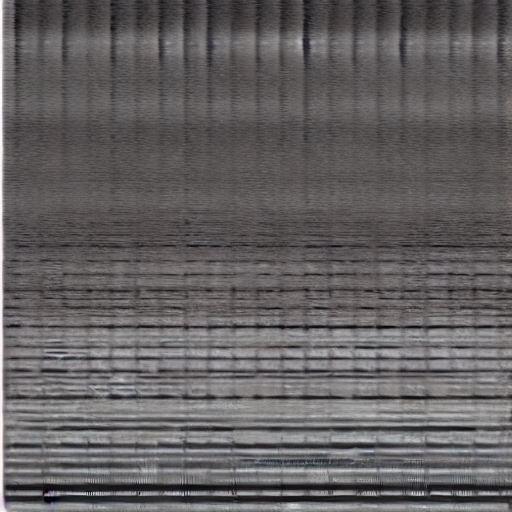
\includegraphics[width=0.8\linewidth]{energy_guitar.jpg}
      \caption{シード値42, テキスト``energy guitar''の入力でRiffusionにより生成されたメルスペクトログラム}
    \label{melsp}
  \end{center}
\end{figure}

そして, メルスペクトログラムに対して逆短時間フーリエ変換を施すことによって波形データが得られ, 
人が音源を聞くことができるようになる.

\newpage
\section{Riffusionの課題}
Riffusionを用いて, ユーザーのイメージする音楽を生成するためには, 
\begin{enumerate}
  \item テキストデータを入力.\label{step1}
  \item Riffusionがメルスペクトログラムを生成, それを音源に変換.
  \item ユーザーが音源を試聴.
  \item もし, 音源がユーザーのイメージでない場合, シード値やテキストデータを変更し, \ref{step1}.から再度生成
\end{enumerate}
という手順を踏む必要がある.

ここで2点の課題が指摘される.
まず, Riffusionには対話機構や前後関係の情報を記録する仕組みがない, すなわち文脈がないため, 2回目以降の生成時に入力テキストが変更されたとしても,
再度生成された音源がイメージに近づく保証はないという点がある.
次に, ユーザーは生成された音源が自分の要求するものであったかを生成される度に確認する必要があり, この作業はユーザーにとって
負担となりうる点である.

これらの課題は, 特に音楽やイラストといった芸術に関する多くの生成AIに共通するものであり, 
改善されることによって, 社会において, より効率的なAI利用を促進することに繋がることが期待される.

\newpage
\chapter{本研究において提案するシステム}
本章では本研究において提案するシステムを発想するに至った先行研究とシステムの概要について述べる.
\section{先行研究}
Riffusionが以前に生成した音源と比較して, よりユーザーのイメージに近い音楽を呈示するための方法として
音源呈示前に, Riffusionとは別の機構によって\dashuline{ユーザーの要求を満たしている\\と期待される音源}
かどうかを予め判定すれば良いと考えた.

Riffusionが他の音楽生成AIと異なる大きな特徴は, 楽曲の生成過程に画像データを経由する点にある.
この画像, メルスペクトログラムから楽曲印象を推論することができれば, 
音源に変換するための時間短縮や, リソースの削減が可能である.

これまでに, スペクトルやスペクトログラムと楽曲印象との相関を分析した研究が数多く報告されている\cite{Nagoya,Tokyo, Matsue}.

これら文献から, メルスペクトログラムから楽曲印象を推論し, 
ユーザーの要求を満足しているかを判定できる可能性は十分にあると考えた.
また, 判定機構には人間の感性を模倣するためにニューラルネットワーク(NN)を用いる.

\newpage
\section{システム概要}
図\ref{system}に本研究で開発した提案するシステムの概要を示す.

\begin{figure}[htbp]
  \centering
  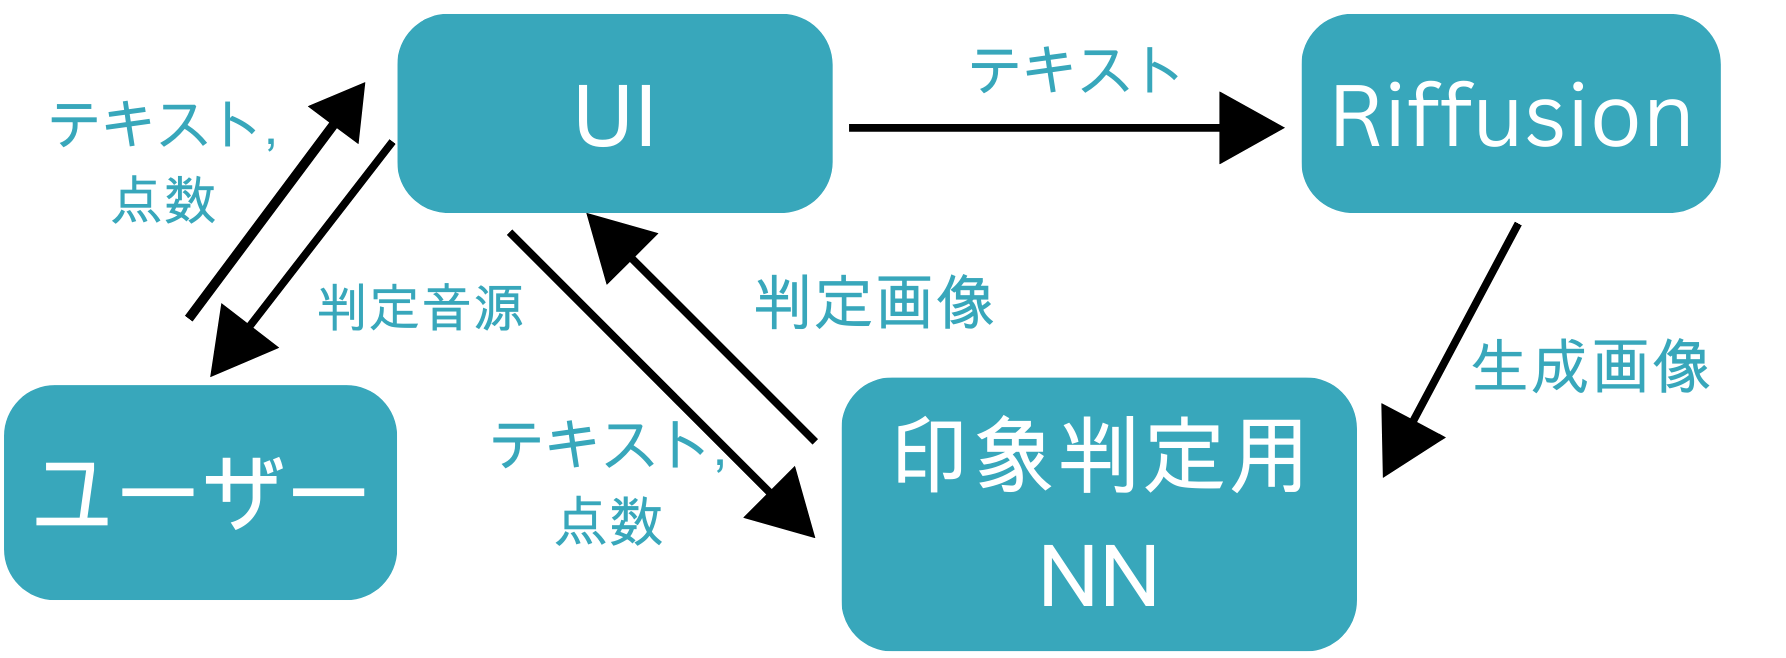
\includegraphics[width=\linewidth]{sys.png}
  \caption{提案システムの概要}
  \label{system}
\end{figure}

システムの動作, すなわちシステムとユーザーの一連の対話は以下の手順になる.
\begin{enumerate}
  \item ユーザーがUIにテキストデータを入力する.\label{s1}
  \item 与えられたテキストからRiffusionがメルスペクトログラムを生成する.\label{s2}
  \item 生成されたメルスペクトログラムを印象判定用NNの入力とし, 判定する.\label{s3}
  \item 印象判定用NNの判定を満たすまで\ref{s2}.,\ref{s3}.を繰り返す.
  \item UIにて判定されたメルスペクトログラムが音源に変換され, 呈示される.
  \item ユーザーは生成された音源を試聴し, 音源から受けた感情に対し, 9つの項目(\ref{GEMS}にて後述)について点数をつける.
\end{enumerate}
また, 3回目以降の対話ではこれまでに生成されたメルスペクトログラムとそれにユーザーがつけた点数を学習データとして,
印象判定用NNに\textbf{転移学習}を行わせる.

転移学習とは, 事前に学習されたNNに対して, 
新たなデータを学習させる際に出力層の形式やパラメータのみを変更することで再学習させる手法である.
この手法により, 転移学習を行ったNNは初め学習していた知識を持ったまま, 
その後のタスクに特化したNNとして振る舞うことが可能である.

本システムでは印象判定用NNが徐々に使用ユーザーに近い感性を学習することを目的に導入した.

\chapter{印象判定用NN}
本章では印象判定用NNに用いたモデルや, データセット, その学習結果について述べる.
\section{DenseNet}
前章にて, スペクトルやスペクトログラムから楽曲印象を推論できる可能性について述べたが, 
これらの研究\cite{Nagoya,Tokyo, Matsue}では, 限定された一部の印象に関する結果や, 線形関数を用いる判別法が
主として用いられており, 人間の感性という複雑な事象への足がかり的なアプローチが多かった.

本研究では, 楽曲から得られるそのような複雑な感性を模倣する必要があることから, NNを用いるに至った.
また, 先行事例のように画像の特徴量から印象を得るため, 畳み込みNN(CNN)を用い, その複雑さに対応するために
多層かつ勾配消失問題への対応がなされているDenseNet\cite{Dense}をアーキテクチャに用いた. 
DenseNetの特筆すべき特徴として, Dense connectivityが挙げられる.
これは, 任意の層の入力をそれ以前の全ての層の出力として, 学習する機構である.
この機構によって, 上で述べたような対応が可能となっている.
DenseNetでは, その他の工夫もなされているが, 今回用いたハイパーパラメータなどの詳細についてはソースコード\ref{source}を参照されたい.
\section{データセット}
印象判定用NNは,初めに\textbf{一般的な感性}によって楽曲を判定し, その後転移学習によって, 感性をパーソナライズ化したいと考えた.
そこで, データセットにはDataset on Induced Musical Emotion from Game with a Purpose Emotifyと呼ばれるA.Aljanakiらが文献\cite{game}にて用いた楽曲400曲と, 同事例で収集された楽曲から感じ取られた印象
に関するアンケート結果を用いた.
\subsection{データセットの特徴}
使用したデータセットの特徴を以下にまとめる.
\begin{itemize}
  \item オンライン上で公開されたゲーム内で, 被験者の対象を性別や年齢, 母国語などによって制限せずに行われた 
        楽曲の印象などについてのアンケート結果である.
  \item 楽曲はrock, classical, pop, electronicの4ジャンル, それぞれ100曲が使用された.
        また, ほとんどの楽曲において1曲あたりの再生時間は1[min]で統一されている. ただし, 一部再生時間1[min]に満たない曲も使用された.
  \item 被験者はゲーム開始前に, ランダムに選択された楽曲を初めから試聴し, \dashuline{9つの感情項目}に関して, 特に強く感じられた項目を
        3項目まで選択した. ただし, 楽曲の試聴に関しては途中でやめてもよいものとしている.
\end{itemize}

このデータセットの特徴として, 被験者の対象を広く設定していることから, 印象判定用NNが一般的な感性を学習することが期待された.

また, 本データセットにおいて, 用いられた9つの感情項目はGEMSを基にした項目となっている.
GEMS(Geneva Emotional Music Scale)\cite{GEMS}とは延べ1000人以上の被験者から得られたアンケート結果に対して, 
因子分析などを行い9つに大別した, 人が音楽から感じる, 誘発される感情のことである.
その9つとはそれぞれ, Wonder, Transcendence, Tenderness, Nostalgia, Peacefulness, Power, 
Joyful activation, Tension, Sadnessとなっている. 
しかし, そのうちTranscendence, Wonder, Peacefulnessは
被験者がその単語の使われ方を正しく理解をすることが困難であった.
そのため, 使用したデータセットではそれぞれについて, Solemnity, Amazement, Calmnessに変更され, 調査が行われた.

\subsection{データセットの作成方法}
前小節で述べた全ての楽曲からメルスペクトログラムを作成した.
作成の際, 以下の2点について考慮した.

一つは, 仮に作成されたメルスペクトログラム中や, 各メルスペクトログラム間に時刻的な重なりがあった場合, 
曲序盤部分および曲終盤部分に対しての\dashuline{学習が曲中盤部分に比べて薄くなる}ことが危惧された点である.
そのような学習データの偏りを軽減させる方法として, 
重なりのない終盤部分を先頭にし, その後同様に重なりのない序盤部分を結合し, メルスペクトログラムを作成することで
曲が繰り返しているようにみなすことも可能であったが, その場合, 印象判定用NNが曲の不連続点を特徴量として学習する恐れや, 
そもそも, 得られたアンケート結果はそのようにして作成された曲を評価したものではなかったため, その方法は不適であると考えた.

また, アンケートの対象者は楽曲を先頭から試聴しており, さらに, 曲の途中で試聴を中断してから回答してもよいことになっていた点である.
このことから, 曲序盤部分の方が, 曲終盤部分に比べてアンケート結果に\dashuline{与えた影響は大きい}と考えられた.

これらのことから, 楽曲からメルスペクトログラムへの変換の際には, 
曲の\textbf{先頭}から, メルスペクトログラム中や, 各メルスペクトログラム間に一切の\textbf{時刻的重なりが生じない}ように注意を払った.
なお, 本研究におけるメルスペクトログラムは1枚あたり5.12[s]の情報を表し, ほとんどの楽曲は1曲1[min]であったため,
1曲あたり11枚のメルスペクトログラムが作成することが可能である.
ただし, 1[min]に満たない楽曲もあったため, 結果としては合計4,380枚のメルスペクトログラムが得られた.
ジャンルごとの枚数の内訳は, rock, pop, electronicは各1,100枚, classicalは1,080枚であった.

次に, 作成されたメルスペクトログラムの正解ラベルに関して, 以下の点を考慮する必要があった.
\begin{itemize}
  \item アンケートにて, 各楽曲に回答した被験者の数や, 項目の選択された数が異なる点.
  \item アンケート結果の上位数項目を正解と限定して, マルチラベル問題とした場合, 人間の感性における微妙なニュアンスが
        推論できないことが危惧される点.
  \item 印象判定用NNが感性を模倣する対象者は個人を想定しているが, 個人が楽曲から得た感情の大小は本データセットからは得られない点. 
\end{itemize}
これらの問題を解決するために, 正解ラベルとして\textbf{単位印象ベクトル}を用いることを提案した.
これは, 各楽曲で得られた項目が選択された数に対し, 大きさが1の単位ベクトルとして正規化を行ったものである.
単位印象ベクトルを用いることによって, 印象の推論を\textbf{9次元単位超球表面上の回帰問題}として扱った. 

正解ラベルに単位ベクトルを用いることは, 
\begin{itemize}
  \item これまで曖昧な事象に対して, マルチラベル分類による二値出力をするような推論を行った結果, 精度が低くなった事例が報告されていた.
        これに対して, 単位ベクトルを出力とすると曖昧な事象に対する\textbf{``方向''}を出力とするため, 従来手法の代替となることが期待される点.
  \item 類似した複数項目の回帰問題に対して1項目ずつ行っていた学習を\textbf{1度}に実施することが可能な点.
\end{itemize}
といった点に対して, NNの推論並びに利用に関して可能性を広げることにつながると考える.

ところで, 補足として本研究では1曲から得られたすべてのメルスペクトログラムに対して同一の正解ラベルが付与されている点に注意されたい.

\section{学習結果}
\label{learning}
前小節のようにして作成されたデータセットを, DenseNetに学習させた.
分割の際に, 各ジャンルの中から無作為に1000枚のメルスペクトログラムを選択し計4,000枚を訓練用データ(train), 残りの380枚を検証用データ(valid)とした.
また, メルスペクトログラムはその方向にも時刻的意味があることから, 学習時にデータ拡張は行っていない.

\newpage
そして, 損失関数には2つの単位ベクトル間の\textbf{距離}である\textbf{二乗平均平方根誤差}(RMSE)を, その他の評価関数には単位ベクトル間の\textbf{角度}(Degree)と, 回帰モデルの指標として用いられる\textbf{R2スコア}($\mathrm{R^2}$)を用いた.
距離, 角度, R2スコアはそれぞれ\ref{RMSE}, \ref{Deg}, \ref{R2}式で表される.
\begin{align}
  \mathrm{RMSE}&= \sqrt{\frac{1}{n} \sum_{i=0}^{n-1} (y_i - \hat{y_i})^2}\label{RMSE} \\ 
  \mathrm{Degree} &= \cos^{-1}{\sum_{i=0}^{n-1}y_i \cdot \hat{y_i}}\label{Deg}\\
  \mathrm{R^2} &= 1 - \frac{\displaystyle \sum_{i=0}^{n-1}(y_i - \hat{y_i})^2}{\displaystyle \sum_{i=0}^{n-1}(y_i - \bar{y})^2}\label{R2}
\end{align}

図\ref{result}に, 300エポック学習した際の損失関数のグラフを示す.

\begin{figure}[htbp]
  \centering
  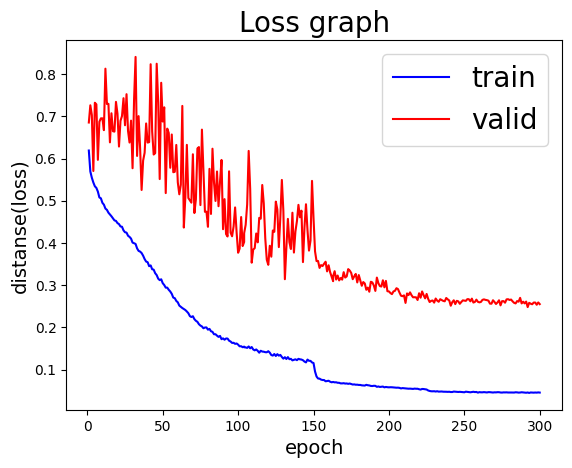
\includegraphics[width=0.8\linewidth]{graph.png}
  \caption{300エポック学習した際の学習用データと検証用データの損失関数の推移}
  \label{result}
\end{figure}

図\ref{result}からエポック数が増えるにつれて徐々に学習が進んでいることが読み取れる.

trainにおける最良値は293エポック目で, RMSE=0.0449, Degree=2.5727, $\mathrm{R^2}$=0.9926であった. この結果から, 距離, 角度に関しては正解ラベルと推論結果がほとんど一致しているといえ, またR2スコアに関しては最高値が1であるため, trainに対する学習はほとんど完了していることがいえるだろう.

そして, validにおける最良値は292エポック目で, RMSE=0.2482, Degree=14.3594, $\mathrm{R^2}$=0.7247であった. この結果から, 距離, 角度に関しては概ね方向が一致しているといえるだろう.また, R2スコアに関しては良いモデルであるということができる.
また, これらからtrainに対して過学習は起きていないと考えられる.

これまでの研究では線形関数的なアプローチが多くなされてきた中で, 本研究の結果として主観的ではあるものの, CNNによって\textbf{人が音楽から感じられる印象について推論ができる可能性}が示唆されたといえるだろう.

\chapter{NN有効性検証実験}
本研究では, 前章にて述べた印象判定用NNの本システムに対する有効性に関して検証実験を行った.
本章では, その概要, 結果, 考察について述べていく.
\section{実験概要}
本実験は, Riffusionによって生成された楽曲が印象判定用NNによって判定されることで, 印象判定用NNが使われない場合と比べて, よりユーザーのイメージに近い楽曲が多く呈示されることを確かめるために被験者を募集し行われ, 彼らの主観評価による結果を用いた.

実験を行う際, 以下のようなバイアスによって正確な実験結果が得られないことが考えられた.
\begin{itemize}
  \item 被験者と実験者の間に繋がりがある場合, 被験者が忖度をし, 実際より良い評価をしてしまう可能性がある点.
  \item 本実験は実験者が実験の補助として実際に立ち会う必要があった. 
        しかし, 被験者が評価する際, そのシステムを制作した実験者が近くにいることを知った場合, 
        実験者に配慮し, 実際より良い評価をしてしまう可能性がある点
  \item 実験内容が``生成された音楽の評価''であると被験者が事前に知っていた場合,
        被験者が実験者に配慮し, 実際より良い評価をしてしまう可能性がある点
\end{itemize}
これらのことから, 被験者は実験者との接点がないことを確認し, 実験内容の詳細は直前まで伏せられ, 
実験中も実験同伴者が実験者であることは伏せながら実験を行った.

次に, 行われた実験の手順を以下に示す.
\begin{enumerate}
  \item 初めに, 被験者はユーザーネームを入力する.
  \item そして, 被験者は生成したいイメージを英語テキストでUIに入力する.
        そのテキストデータから, 無作為なシード値が設定されたRiffusionは音源を1つ生成する.
        音源はUIにて呈示され, 被験者はその音源を試聴し, そこから受けた印象についてデータセットで用いられた9項目, すなわち一部改変されたGEMSに沿って採点を行う.
        この際, 図\ref{UI1}のように, 1項目につき0-100点をスライダー形式を用いて\textbf{採点}を行った. なお, その項目の感情を強く感じた場合に100点をつけるよう, 被験者には伝えた.\label{exp1}
  \item 次に被験者は, \ref{exp1}.において生成された音源に対して
        より\dashuline{被験者のイメージに近づくような\\英単語}を, 
        \ref{exp1}.のテキスト中の英文法上適切な位置に1語のみ追加しUIに入力する.
        システムはこのテキストから, \ref{exp1}.で用いたシード値に1,2,3だけ加算したシード値を設定し, 音源をそれぞれ生成する. この3つの音源はNNによる判定を通していないダミー音源として, 対照実験に用いる. そして, 印象判定用NNによって判定された音源が3つになるまで, ダミー音源を生成する際に使ったシード値に1ずつ加算し, 同テキストから音源を生成, 印象判定用NNによる判定を繰り返す. こうして生成された6つの音源はランダムな順でUIにて被験者に呈示される. 被験者は各音源に対してまず, \ref{exp1}.で生成された音源と比べて\textbf{自分のイメージに近かったか}を回答し, 次に, \ref{exp1}.と同様にGEMSに沿った\textbf{採点}を行った.\label{exp2}
  \item 次に被験者は\ref{exp2}.で用いたテキストをUIに入力する.
        システムは\ref{exp2}.と同様に\ref{exp2}.終了時点のシード値に1,2,3を加算したシード値を設定し, ダミー音源を3つ生成する.
        ところで, この時点までにシステムには, \ref{exp1}.,\ref{exp2}.において生成された7つのメルスペクトログラムとそれぞれに対して正規化された採点結果が記録されている.
        ダミー音源生成終了後, それらを学習データとして用い, 印象判定用NNに対して転移学習を行わせる. そうしてできた転移学習済印象判定用NNによる判定によって, ダミー音源生成時のシード値に1だけ加算したシード値を初めの値として, \ref{exp2}.と同様に音源を3つ生成する.
        その後, UIにてランダムな順で6つの音源が呈示され, \ref{exp2}.と同じ項目について, 被験者は回答, 採点を行った.\label{exp3}
  \item 最後に, 被験者は任意で感想を入力する.
\end{enumerate}

\begin{figure}[htbp]
  \centering
  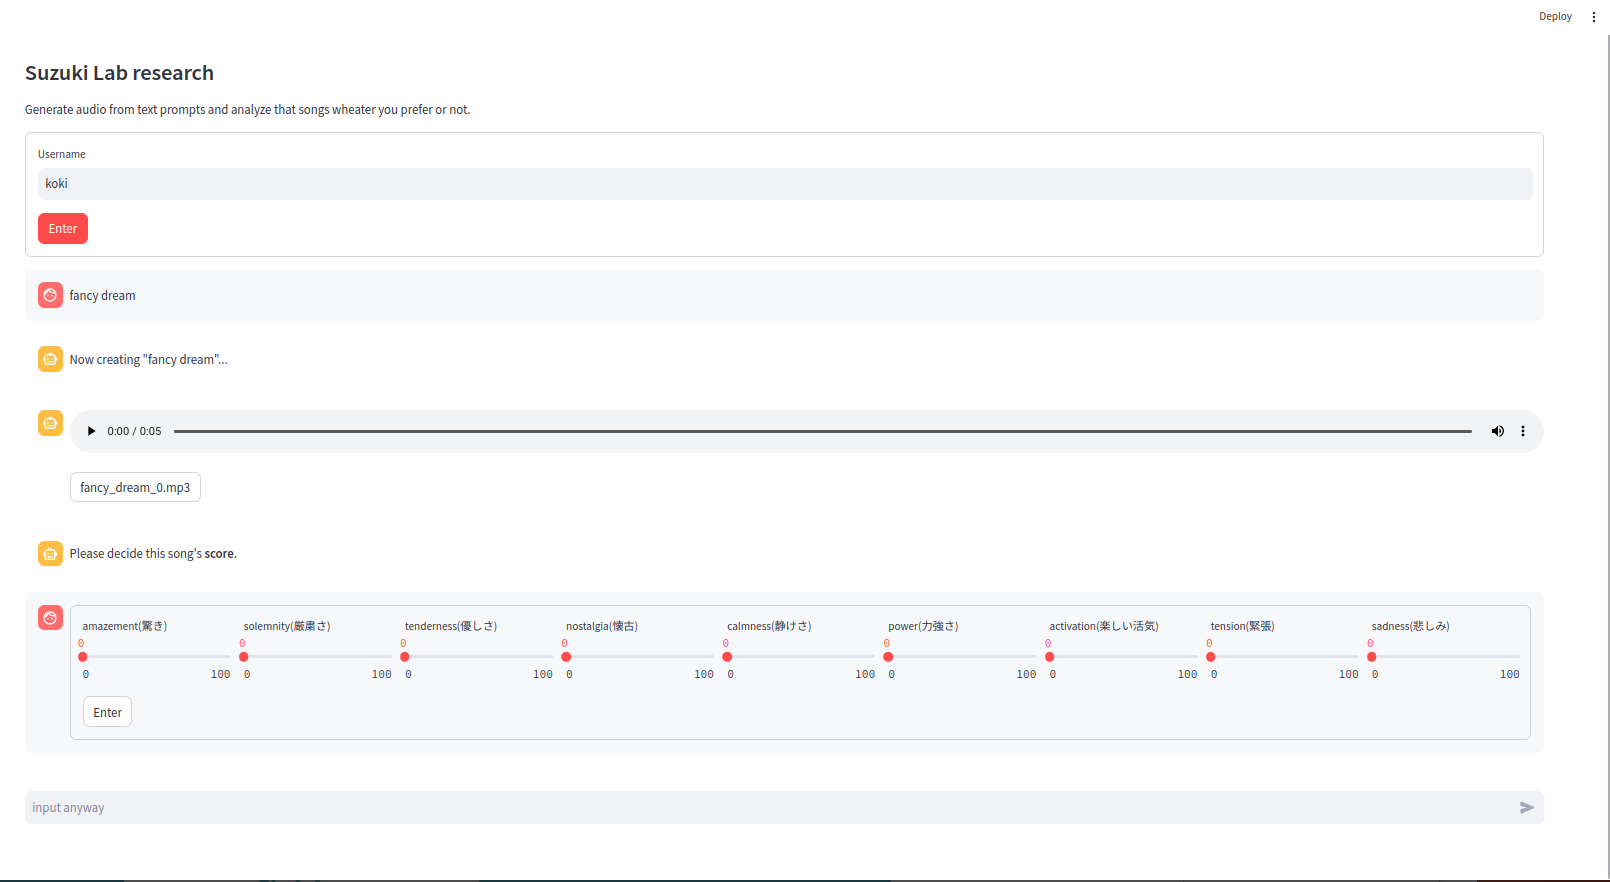
\includegraphics[width=0.9\linewidth]{UI.png}
  \caption{本実験に用いたUI画面}
  \label{UI1}
\end{figure}

図\ref{UI1}のUIにはPythonライブラリであるStreamlit\cite{stream}を用いた.
これはWebアプリの作成が可能なフレームワークである. 
キャッシュ機能や状態保存機能を備えていることから機械学習を用いた簡易アプリケーションを作成する際に重宝される.

本実験における印象判定用NNには, \ref{learning}の検証用データにて最良値であった292エポック目のパラメータを用いた.
また, 手順\ref{exp2}.は``一般的な感性''が期待されるNNによる有効性を, 手順\ref{exp3}.は``ユーザーの感性''にパーソナライズ化されたことが期待されるNNの有効性を検証する目的で行われた.
手順\ref{exp3}.における転移学習は40エポックで行っており, その50\%である20エポック目, 75\%である30エポック目ではそれぞれ学習率を0.1ずつ減衰させた.


当実験ではその手法上, 被験者によってはダミー音源が偶然, イメージに近い音源ばかりを生成する可能性があった.
そのような外れ値を軽減するため, できる限り被験者の母数を多くする必要があった.
本実験は, そのような背景の中, 釧路工業高等専門学校の学生11名の協力の元, 実施された.
被験者の構成としては, 本科1年生5名, 2年生1名, 3年生1名, 4年生3名, 専攻科1年生1名, 全員男性となっている.

また, 今回の実験における``判定''は, 以下のように行われている.
\begin{enumerate}
  \item 追加された1語について, Word2Vec事前学習モデルを用い, 
        データセットの9項目それぞれの単語との類似度を測定する.
  \item 類似度の値が最も高かった項目について, 
        実験手順\ref{exp1}.で生成された音源の値と実験手順\ref{exp2}. , \ref{exp3}.で生成された音源の値で比較を行い, 後者の値が大きかった場合, 
        判定された音源とした.
\end{enumerate}
なお, Word2Vec事前学習モデルには英語版wikipediaから学習された100次元モデル\cite{NLP}を使用した.

\section{実験結果}
表\ref{table}に, 前節実験手順\ref{exp2}. , \ref{exp3}.で生成されたダミー, 判定音源の, 実験手順\ref{exp1}.で生成された音源よりイメージに近かった全被験者における総和を示す.

\begin{table}[htb]
  \caption{実験手順\ref{exp2}. , \ref{exp3}.における被験者のイメージに近かったダミー, 判定音源の総和}
    \label{table}
    \vspace{2mm}
    \begin{center}
        \begin{tabular}{|c|c|c|c|}
            \hline
            \multicolumn{2}{|c|}{実験手順\ref{exp2}.}&\multicolumn{2}{|c|}{実験手順\ref{exp3}.}\\
            \hline
            ダミー音源 & 判定音源 & ダミー音源 & 判定音源\\
            \hline
            23 & 23 & 22 & 21\\
            \hline
        \end{tabular}
        \end{center}
\end{table}

なお, 表\ref{table}の各音源の総和は生成された各項目の音源の総和33曲の中から回答された数であることに注意されたい.
表\ref{table}より, 各手順におけるダミー音源の数と比較して, 判定された音源の数は横ばい, または僅かに減少していることが見られる.

\section{実験結果に対する考察}
前節の結果から, 本研究で作成した印象判定用NNには, 転移学習の有無を問わずRiffusionから生成された音源に対し, ユーザーのイメージに近い音源を呈示する有効性が見られなかった.
この結果となった原因として, 以下の点が考えられる.
\begin{itemize}
  \item 印象判定用NNの学習データがrock, classical, pop, 
        electronicの4ジャンルしかなく, Riffusionが生成しやすい
        楽曲のジャンルと一致しなかった可能性がある点.
  \item ``判定''における自然言語処理が単純な処理であり, 正しい判定がなされなかった可能性がある点.
\end{itemize}

まず一つ目の点について, 4ジャンルではRiffusionが生成する楽曲の幅に対して, 学習が不足している可能性が指摘される.
また, 主観的な見解としてRiffusionは高い頻度で, 楽曲とは言い難いノイズのような音源を生成する. 
今回の実験では, ノイズを求めるようなイメージのテキストは存在しなかった.
しかし, 実際には何度もノイズのような音源が呈示されていた.
印象判定用NNの学習データにはノイズのような音源はなかったため, 結果としてノイズも音源として認識してしまい, 判定されたことも原因として考えられる.

次に二つ目の点については, 今回の``判定''の対象にした単語が追加された1語のみであったことが一つの理由として挙げられる.
さらに, 単語の類似度で最も高い項目のみについて比較を行ったことが, ベクトル空間による推論の優位性を損ねてしまったことも実験結果に大きく寄与してしまった要因として想定される.

\newpage
\chapter{システム実証}
本章では, 前章と並行して行ったシステム実証についてその概要, 結果, 考察を述べる.
\section{実証概要}
本実証は提案した対話型楽曲生成システムの開発意義の有無を検証することを目的に行われた.
また, 本実証は釧路工業高等専門学校の学生7名に協力を仰ぎ, 実施された.
学生の内訳は, 本科5年生7名, 男性6名, 女性1名である.
これら被験者は実験者が協力を募り, 参加していることに注意されたい.

本実証は以下の手順で行われた.
\begin{enumerate}
  \item 初めに, 被験者はユーザーネームを入力する.
        この際, システムによって無作為にシード値が決定される.
  \item 次に, 被験者は生成したい楽曲のイメージをテキストとして入力する.
        この入力時点でのシード値から1ずつシード値を加算し,
        音源を5つ生成する.それらの印象判定用NNによる推論の平均値を正規化した値を
        印象判定の基準として, 以降判定された音源が生成されるまでシード値を1ずつ加算し, 
        音源を生成する. その後, UIにて判定された音源を呈示され, その音源に対し被験者は
        データセットで用いた9項目(一部改変されたGEMS)について前章の実験と同様に採点を行う.
        この手順\ref{sys2}.を以後対話と呼ぶ.
        \label{sys2}
  \item 各対話ごとに被験者は任意のテキストを入力し, 対話を計7回繰り返した後, 
        「システムは徐々にあなたのイメージした楽曲を呈示するようになったか」と
        UI上にて質問される.
        これに対し,被験者はYes/Noで回答をした.
  \item 最後に, 被験者は任意で感想を入力した.
\end{enumerate}

本実証のUIには, 前章同様Streamlitが用いられた.

また, 本実証での印象判定用NNには, 前章と同じく\ref{learning}の検証用データにて最良値であった292エポック目のパラメータを用いた.

1,2回目の対話では印象判定用NNをそのまま, それ以降の対話ではそれ以前に得られた全てのメルスペクトログラム, 正規化された点数を用いて転移学習された印象判定用NNを用いて判定が行われている.

今回の実証における``判定''は, 以下のように行われている.
\begin{enumerate}
  \item 入力されたテキスト中の単語で, 使用したWord2Vec事前学習モデル内に存在する単語に関して, 
        データセットの9項目それぞれの単語との類似度を測定する.
  \item 各単語について類似度の値が最も高かった項目を集計し, 
        最もその単語数が多かった項目に関して, 
        基準となる値と新たな生成された音源の値で比較を行い, 後者の値が大きかった場合, 
        判定された音源とした.なお, 最多単語数が複数項目において同数だった場合には, 生成された音源の値が過半数の項目で基準を上回った際に判定された音源とした.
\end{enumerate}
ここで, Word2Vec事前学習モデルには前章と同様のものを使用した.

\section{実証結果}
本実証での7回の対話後の質問に対して, 7名中5名がYes, 2名がNoと回答した.
これは71\%の被験者が徐々に感性にあった楽曲を呈示するように感じたことを表している.

\section{実証結果に対する考察}
前節の結果に対する見解として, 対話型楽曲生成システムの開発意義に関して否定することはできないとするのが妥当であると考える.
一方で, 前章の結果から印象判定用NNや転移学習には本システムに対する有効性が見られなかったにも関わらず, このような結果が得られたことについて, 以下のような可能性が考えられる.
\begin{itemize}
  \item システムが期待通りの振る舞いをするはずであるという思い込みによって実情よりも良い評価がされた可能性.
  \item 被験者が実験者と接点がある学生であったことから, 実験者に配慮されてしまい, 実情よりも良い評価がされた可能性.
  \item ``判定''に用いる単語をテキスト中の全単語に範囲を広げたことによって, より正確な判定を行えるようになった可能性.
\end{itemize}
これらのことから, 本システムの開発意義や性能改善に関して今後, より慎重に精査をする必要があると考える.

\chapter{結論}
本研究ではRiffusionを用いて対話型プロンプトによる音楽生成システムの開発を目指し, 取り組んだ.
そのシステムにおいて, ユーザーが自分のイメージに近い楽曲を生成するためにCNNを用いることで, 性能向上を図った.
その結果として, まず, CNNによる\textbf{人が音楽から受ける感情の推論可能性}が示唆された.
そして, 対話型楽曲生成システムの\textbf{開発意義に関しては否定できないこと}が判明した.

本研究の今後の課題としては, 以下の3点が考えられる.
\begin{enumerate}
  \item 印象判定用NNの学習データの拡充
  \item 判定における自然言語処理方法の変更
  \item 被験者数の小規模さ, 被験者の年代
\end{enumerate}

1つ目の点について, 今回の実験では印象判定用NNが本システムの性能向上に有効性が見られなかった.
そのため, 対応策として, 学習データのジャンルやデータ数を拡充することで, より汎用的な推論を可能にしたいと考えている. また, その具体的な手法としては本システムをオンライン上で公開することで, データを収集することを現状考案している.

2つ目の点について, 今回の実験の処理方法では単位ベクトルを用いた利点として期待された無視されがちな微小な感性の表現に関して有効活用することができなかった. その改善方法として, 各項目の類似度による重みづけを用いた判定について模索, 検討を行っている. 

3つ目の点について, 今回の実験, 実証の被験者は延べ18名の学生であり, 比較的小規模かつ年代に偏りが生じてしまった. そのため, 正確な実験, 実証結果であったかは疑念が拭えないものとなっている. 今後の展望として, 1つ目に挙げたようにオンラインによる調査を行うことによって, より正確で幅広い結果が得られることを期待している.

今後は以上の点を考慮しつつ, 対話型楽曲生成システムの性能向上を目指す.

\chapter*{謝辞}
本研究を遂行するにあたり, ご指導並びにご助力いただいた鈴木未央教員に感謝申し上げます.
また, 実験に協力いただいた学生の皆さま, そして, 日常の議論を通じ多くの知識, 発見, 示唆をいただいた鈴木研究室の皆さまに深くお礼申し上げます.
\addcontentsline{toc}{chapter}{\numberline{}謝辞}

\newpage

\chapter*{付録}
\addcontentsline{toc}{chapter}{\numberline{}付録}
\section*{印象判定用NNソースコード}
\addcontentsline{toc}{section}{\numberline{}印象判定用NNソースコード}
\begin{lstlisting}[caption=印象判定用NN{,} DenseNetに関するソースコード, label=source]
  import torch
  import torch.nn as nn
  import torch.optim as optim
  
  import pytorch_lightning as pl
  from torchmetrics.regression import R2Score
  import numpy as np
  
  
  class Degree(nn.Module):#θと内積です
      def __init__(self): # パラメータの設定など初期化処理を行う
          super(Degree, self).__init__()
  
      def forward(self, outputs, targets): # モデルの出力と正解データ
          loss = torch.mean(torch.rad2deg(torch.acos(torch.sum(outputs*targets, dim=-1, keepdim=True))))
          return loss
  
  class RMSELoss(nn.Module):
      def __init__(self): # パラメータの設定など初期化処理を行う
          super(RMSELoss, self).__init__()
  
      def forward(self, outputs, targets): # モデルの出力と正解データ
          loss = torch.mean(torch.norm(outputs - targets, dim=-1))
          return loss
  
  class Vectolize(nn.Module):
      def __init__(self):
          super(Vectolize, self).__init__()
  
      def forward(self, in_channels):
          in_channels = torch.abs(in_channels)
          unit_vector = in_channels / torch.norm(in_channels, dim=-1, keepdim=True)
          return unit_vector
  
  
  class bn_relu_conv2d(nn.Module):
      def __init__(self, in_channels, out_channels, kernel_size, stride,padding=1):
          super(bn_relu_conv2d, self).__init__()
          self.bn = nn.BatchNorm2d(in_channels)
          self.relu = nn.ReLU(inplace=True)
          self.conv = nn.Conv2d(in_channels, out_channels, kernel_size=kernel_size, stride=stride, padding=padding)
          self.drop = nn.Dropout(0.2)
  
      def forward(self, x):
          out = self.bn(x)
          out = self.relu(out)
          out = self.conv(out)
          out = self.drop(out)
          return out
  
  class bn_relu_conv1d(nn.Module):
      def __init__(self, in_channels, out_channels, kernel_size, stride,padding=1):
          super(bn_relu_conv1d, self).__init__()
          self.bn = nn.BatchNorm1d(in_channels)
          self.relu = nn.ReLU(inplace=True)
          self.conv = nn.Conv1d(in_channels, out_channels, kernel_size=kernel_size, stride=stride, padding=padding)
          self.drop = nn.Dropout(0.2)
  
      def forward(self, x):
          out = self.bn(x)
          out = self.relu(out)
          out = self.conv(out)
          out = self.drop(out)
          return out
  
  class dense_layer(nn.Module):
      def __init__(self, in_channels, growth_rate):
          super(dense_layer, self).__init__()
  
          self.conv1 = bn_relu_conv2d(in_channels, out_channels=growth_rate*4, kernel_size=1, stride=1, padding=0)
          self.conv2 = bn_relu_conv2d(growth_rate*4, out_channels=growth_rate, kernel_size=3, stride=1)
  
      def forward(self, x):
          out = self.conv1(x)
          out = self.conv2(out)
          return out
  
  class dense_block(nn.Module):
      """dense block"""
      def __init__(self, in_channels, num_layers, growth_rate):
          super(dense_block, self).__init__()
  
          dense_layers = []
          for i in range(num_layers):
              dense_layers += [dense_layer(in_channels=int(in_channels + i*growth_rate), growth_rate=growth_rate)]
          self.dense_layers = nn.Sequential(*dense_layers)
  
      def forward(self, x):
          for layer in self.dense_layers:
              out = layer(x)
              x = torch.cat([x, out], 1)
          return x
  
  class transition_layer(nn.Module):
      def __init__(self, in_channels, out_channels):
          super(transition_layer, self).__init__()
          self.conv = bn_relu_conv2d(in_channels=in_channels, out_channels=out_channels, kernel_size=1, stride=1,padding=0)
          self.pool = nn.AvgPool2d(kernel_size=2, stride=2)
  
      def forward(self, x):
          out = self.conv(x)
          out = self.pool(out)
          return out
  
  class dense_net(nn.Module):
      """dense block"""
      def __init__(self, num_layers, growth_rate, num_classes=1000):
          super(dense_net, self).__init__()
  
          in_channels=  2 * growth_rate
          self.first_layer = nn.Sequential(
              *[bn_relu_conv2d(in_channels=1, out_channels=in_channels, kernel_size=9, stride=2, padding=4),
              nn.MaxPool2d(kernel_size=3, stride=2, padding=1)]
          )
          layer_dense = []
          for i in range(len(num_layers)):
              layer_dense += [dense_block(in_channels=in_channels, num_layers=num_layers[i], growth_rate=growth_rate)]
  
              in_channels += growth_rate * num_layers[i]
              if i != (len(num_layers)-1):
                  layer_dense += [transition_layer(in_channels=in_channels, out_channels=in_channels//2)]
                  in_channels = in_channels//2
  
          layer_dense += [nn.AdaptiveAvgPool2d((1,1))]
  
          self.layer_dense = nn.Sequential(*layer_dense)
          self.fully_connection = nn.Linear(in_channels, num_classes)
          self.classifier = Vectolize()
  
      def forward(self, x):
          out = self.first_layer(x)
          out = self.layer_dense(out)
          out = out.view(out.shape[0], -1)
          out = self.fully_connection(out)
          out = self.classifier(out)
          return out
  
  class DenseTrainer(pl.LightningModule):
      def __init__(self):
          super().__init__()
          self.model = dense_net(num_layers=[6,12,48,32,32], growth_rate=12, num_classes=9) if model is None else model
  
          self.training_step_outputs = []   # save outputs in each batch to compute metric overall epoch
          self.val_step_outputs = []        # save outputs in each batch to compute metric overall epoch
      def forward(self, x):
          out = self.model(x)
          return out
  
      def training_step(self, batch, batch_idx):
          x, y = batch
          x, y = x.to("cuda"), y.to("cuda")
          y_hat = self.forward(x)#hatは予測値
          loss = RMSELoss()(y_hat, y)
          ret = {'loss': loss, 'y_hat':y_hat, 'y':y, 'tr_batch_loss': loss.item()*x.size(0)}
          self.training_step_outputs.append(ret)
          return ret
  
      def validation_step(self, batch, batch_idx):
          x, y = batch
          x, y = x.to("cuda"), y.to("cuda")
          y_hat = self.forward(x)
          loss = RMSELoss()(y_hat, y)
          ret = {'y_hat':y_hat, 'y':y, 'val_batch_loss': loss.item()*x.size(0)}
          self.val_step_outputs.append(ret)
          return ret
  
      def on_train_epoch_end(self):
          y_hat = torch.cat([val['y_hat'] for val in self.training_step_outputs], dim=0)
          y = torch.cat([val['y'] for val in self.training_step_outputs], dim=0)
          epoch_loss = sum([val['tr_batch_loss'] for val in self.training_step_outputs])/y_hat.size(0)
          r2 = R2Score(num_outputs=9, multioutput='raw_values').to("cuda")(y_hat, y).mean()
          mse = Degree()(y_hat, y)
          self.log('train_loss', epoch_loss, prog_bar=True, on_epoch=True)
          self.log('train_r2', r2, prog_bar=True, on_epoch=True)
  
          print('train Loss: {:.4f} train R2: {:.4f} train degree {:.4f}\n'.format(epoch_loss,r2, mse))
  
          self.training_step_outputs.clear()
          
  
      def on_validation_epoch_end(self):
          y_hat = torch.cat([val['y_hat'] for val in self.val_step_outputs], dim=0)
          y = torch.cat([val['y'] for val in self.val_step_outputs], dim=0)
          epoch_loss = sum([val['val_batch_loss'] for val in self.val_step_outputs])/y_hat.size(0)
          print(y_hat[0])
          print(y[0])
          r2 = R2Score(num_outputs=9, multioutput='raw_values').to("cuda")(y_hat, y).mean()
          mse = Degree()(y_hat, y)
          self.log('val_loss', epoch_loss, prog_bar=True, on_epoch=True)
          self.log('val_r2', r2, prog_bar=True, on_epoch=True)
  
          print(f'---------- Current Epoch {self.current_epoch+1} ----------')
          print('valid Loss: {:.4f} valid R2: {:.4f} valid degree: {:.4f}'.format(epoch_loss,r2, mse))
          print()
          self.val_step_outputs.clear()
          
  
  
      def configure_optimizers(self):
          optimizer = optim.SGD(self.parameters(), lr=0.01, momentum=0.9, weight_decay=1e-4)
          scheduler = torch.optim.lr_scheduler.MultiStepLR(optimizer, milestones=[150, 225], gamma=0.1)
          return {'optimizer': optimizer, 'lr_scheduler': scheduler}
  
  
  
  class TransferTrainer(pl.LightningModule):
      def __init__(self, model):
          super().__init__()
          self.model = model
          self.model.train()
          for param in self.model.parameters():
              param.requires_grad = False
          
          self.model.fully_connection = nn.Linear(744, 9)
  
          self.training_step_outputs = []   # save outputs in each batch to compute metric overall epoch
  
      def forward(self, x):
          out = self.model(x)
          return out
  
      def training_step(self, batch, batch_idx):
          x, y = batch
          x, y = x.to("cuda"), y.to("cuda")
          y_hat = self.forward(x)#hatは予測値
          loss = RMSELoss()(y_hat, y)
          ret = {'loss': loss, 'y_hat':y_hat, 'y':y, 'tr_batch_loss': loss.item()*x.size(0)}
          self.training_step_outputs.append(ret)
          return ret
  
  
      def on_train_epoch_end(self):
          y_hat = torch.cat([val['y_hat'] for val in self.training_step_outputs], dim=0)
          y = torch.cat([val['y'] for val in self.training_step_outputs], dim=0)
          epoch_loss = sum([val['tr_batch_loss'] for val in self.training_step_outputs])/y_hat.size(0)
          r2 = R2Score(num_outputs=9, multioutput='raw_values').to("cuda")(y_hat, y).mean()
          mse = Degree()(y_hat, y)
          self.log('train_loss', epoch_loss, prog_bar=True, on_epoch=True)
          self.log('train_r2', r2, prog_bar=True, on_epoch=True)
  
          print('train Loss: {:.4f} train R2: {:.4f} train MLSE: {:.4f}\n'.format(epoch_loss,r2, mse))
  
          self.training_step_outputs.clear()
  
  
  
      def configure_optimizers(self):
          optimizer = optim.SGD(self.parameters(), lr=0.1, momentum=0.9, weight_decay=1e-4)
          scheduler = torch.optim.lr_scheduler.MultiStepLR(optimizer, milestones=[20, 30], gamma=0.1)
          return {'optimizer': optimizer, 'lr_scheduler': scheduler}
\end{lstlisting}
\newpage
\addcontentsline{toc}{chapter}{\numberline{}参考文献}
\renewcommand{\bibname}{参考文献}

%% 参考文献に jbibtex を使う場合
%\bibliographystyle{junsrt}
%\bibliography{samplebib}
%% [compile] jbibtex sample; platex sample; platex sample;

%% 参考文献を直接ファイルに含めて書く場合
\begin{thebibliography}{1}
\bibitem{Riffuse}
\newblock Riffusion,
\newblock \url{github.com/riffusion}

\bibitem{Diffuse}
\newblock Stability AI,
\newblock \url{ja.stability.ai/stable-diffusion}

\bibitem{trans}
A. Vaswani,
\newblock N. Shazeer,
\newblock N. Parmar,
\newblock J. Uszkoreit,
\newblock L. Jones,
\newblock A. N. Gomez,
\newblock L. Kaiser,
\newblock I. Polosukhin.
\newblock Attension Is All You Need.
\newblock \url{arxiv.org},
\newblock arXiv:1706.03762v7, 
\newblock 2023.

\bibitem{Nagoya}
伊藤 雄哉, 
\newblock 山西 良典,
\newblock 加藤 昇平,
\newblock 伊藤 英則.
\newblock 楽曲に対する感性評価と音響ゆらぎ特徴の対応付け.
\newblock 日本感性工学会論文誌 Vol.10 No.3,
\newblock pp.341-348, 
\newblock 2011.

\bibitem{Tokyo}
宮谷 大輝,
\newblock 中山 英樹.
\newblock スペクトログラム画像を用いた楽曲印象分類による時間及び周波数情報と印象の関係分析手法の提案.
\newblock 情報処理学会研究報告,
\newblock 2015-MUS-106,
\newblock pp.1-5, 
\newblock 2015.

\bibitem{Matsue}
佐々木 翔一,
\newblock 加藤 聡.
\newblock スペクトログラムと自己組織化マップを用いた楽曲分類に関する研究.
\newblock 第36回ファジィシステムシンポジウム 講演論文集(FSS2020 オンライン),
\newblock pp.301-302, 
\newblock 2020.

\bibitem{Dense}
G. Huang,
\newblock Z. Liu,
\newblock L. v. d. Maaten,
\newblock K. Q. Weinberger.
\newblock Densely Connected Convolutional Networks.
\newblock \url{arxiv.org},
\newblock arXiv:1608.06993v5, 
\newblock 2018.

\bibitem{game}
A. Aljanaki,
\newblock F. Wiering,
\newblock R. C. Veltkamp.
\newblock Studying emotion induced by music through a crowdsourcing game.
\newblock Information Processing \& Management, 
\newblock 2015.

\bibitem{GEMS}
M. Zentner,
\newblock D. Grandjean,
\newblock K. R. Scherer.
\newblock Emotions evoked by the sound of music.
\newblock Characterization, classification, and measurement.
\newblock Emotion, 8(4),
\newblock 494-521,
\newblock 2018.

\bibitem{stream}
\newblock Streamlit,
\newblock \url{streamlit.io}

\bibitem{NLP}
\newblock Wikipedia2Vec,
\newblock \url{wikipedia2vec.github.io/wikipedia2vec/pretrained/}

\end{thebibliography}

\end{document}